% ******************************************************************************
% File name: Documentation.tex
% Title:   Documentation for Transfer Limits Animation
% Subject: Documentation based on referencing portions of listing
%
% Created: June 11, 2017
% Original Issue: Pending
% Last Edited: June 11, 2017
% Latest Rev. #: 0
%
% Ref. Docs.:
%
% Revision Notes:
% Rev.0 (June 11/2017 by JZB) Template
% ******************************************************************************
%
%        1         2         3         4         5         6         7         8
% 345678901234567890123456789012345678901234567890123456789012345678901234567890
%

\documentclass[12pt]{report}

% List of all packages is included here
% ******************************************************************************
% File name: Packages.tex
% Title: Preamble material to siplify latex code
% Subject: Commonly used packages to simplify code
%
% Created: July 6, 2010
% Original Issue: 1
% Last Edited: July 14, 2017
% Latest Rev. #: 2
%
% Ref. Docs.:
%
% Revision Notes:
% Rev 2 (07/14/17 by JZB)
% Rev
% Rev.1 (07/06/10 by JB) Original issue
% Use with \input command from the main tex file.
% ******************************************************************************

\usepackage{color} % Enables use of color

\usepackage{listings} % Enables including source code with automatic
                      % syntax higlighting.
\definecolor{dkgreen}{rgb}{0,0.6,0}
\definecolor{gray}{rgb}{0.5,0.5,0.5}
\definecolor{mauve}{rgb}{0.58,0,0.82}

\lstset{ %
  keywordstyle=\color{blue},          % keyword style
  commentstyle=\color{dkgreen},       % comment style
  stringstyle=\color{mauve},         % string literal style
  tabsize=4,
  linewidth=\textwidth,
  breaklines=true,
  breakatwhitespace=false,        % sets if automatic breaks should only happen at whitespace
  numbers=left,
  stepnumber=1,
  basicstyle=\small,
  % caption={\lstname},
  % title=\lstname,
}

\usepackage[nottoc]{tocbibind} % Places bibliography, index, list of figures, and list of tables into TOC

\usepackage{algorithmic} % Enables algorithmic typesetting

\usepackage{verbatim} % Enables usage of quoted text, i.e., computer code.

\usepackage{graphicx}
\usepackage{subcaption}
\captionsetup[table]{textfont=it,position=top}

% Using this together with subfig requires adjustments that I don't
% have time to study.
% \usepackage[justification=centering]{caption}[2007/12/23]
\usepackage[font={small,bf}, justification={centering}]{caption}

%\usepackage{pdfpages} % Enables including pages from pdf documents, must use pdflatex

% Formating of tables
\usepackage{booktabs} % better layout for tables
\usepackage{tabularx} % adds stretching of table columns to fill space
\renewcommand{\arraystretch}{1.5} % adds spacing to table rows

% % Page layout and header/footer
% % \usepackage{fullpage} % Uses the page with reduced margins ~1in all around
% \usepackage{fancyhdr} % Configurable headers and footers
% \setlength{\headheight}{2ex} % Prevents a warning from Latex
% \pagestyle{fancy} % part of the fancyhrd preamble
%
% \usepackage{currfile} % Adds file name and dir to available variables
%                   % (used in header)

\usepackage{setspace} % Adds precise control of paragraph spacing
                      % (used here to format Proprieatry notice)

\usepackage{lastpage} % Adds total page count (used for Page n of N)

% Adding cross references to a pdf file (does not work act in draft mode)
% \usepackage[dvipdfm,hidelinks]{hyperref} % option supports dvi->pdf route
% \usepackage{hyperref} % uses outlines for links, the default outline color is red.
\usepackage[hidelinks]{hyperref} % hides the outlines, but keeps the links active

\usepackage[acronym,toc,nonumberlist,nopostdot,nogroupskip]{glossaries} % Allows for list of acronyms
% \newacronym[longplural=Frames per Second]{fpsLabel}{FPS}{Frame per Second}
\newacronym{acr:PDF}{PDF}{Probability Density Function}
\newacronym{acr:POA}{POA}{Plane of Array}
\newacronym{acr:PSLF}{PSLF}{Positive Sequence Load Flow - GE }
\newacronym{acr:PGnE}{PG\&E}{Pacific Gas and Electric Company}
\newacronym{acr:PV}{PV}{photovoltaic}
\newacronym{acr:NREL}{NREL}{National Renewable Energy Laboratory}
\newacronym{acr:WECC}{WECC}{Western Electric Coordinating Council}
\newacronym{acr:DG}{DG}{distributed generation}
\newacronym{acr:GIS}{GIS}{geographic information system}

% Settings for TOC
% \usepackage[nottoc,chapter]{tocbibind} % Places bibliography, index, list of figures, and list of tables into TOC
% \settocbibname{References}
% \renewcommand{\bibname}{References} %

% \renewcommand{\contentsname}{Table of Contents} %

% \pagenumbering{roman} % writes page numbers in roman (not arabic) numerals

%\linespread{1.6} % Sets line spacing to double (crude)
\usepackage{setspace} % line spacing to double, refined
\singlespacing
%\onehalfspacing
%\doublespacing
% \setstretch{1.1} % use to set a custom one

\usepackage{amsmath}

\usepackage{enumitem} % allows style definition for lists

% \usepackage[margin=1in]{geometry}


\renewcommand\lstlistlistingname{List of Listings}

\makeindex

\title{Transfer Limits Animation}
\author{Jovan Bebi\'{c}\\[0.5ex]
        Marija Bebi\'{c}}

\begin{document}
\pagenumbering{roman} % Changes page numbering to roman
\maketitle

\begin{abstract}
This document is a LaTeX template for creating code documentation. It is typeset
\emph{report} document class, which means that it has chapters and sections.
The main purpose of the document is to illustrate it's use of figures and listings,
but it also showcases cross referencing bibliography entries, etc.
\end{abstract}

\pagenumbering{arabic} % Returns to arabic page numbering
\section*{Revision Notes}
\begin{tabularx}{\textwidth}{|p{1in}|l|c|X|}
\hline
Authors & Date & Rev & Notes \\
\hline
JZB & Jun 11-14, 2017 & Draft & Template for use by others \\
\hline
\end{tabularx}

\tableofcontents
\listoffigures
\addcontentsline{toc}{chapter}{\lstlistlistingname}{\lstlistoflistings}

\doublespacing
\chapter{Introduction}
\label{ch:intro}
This is a template LaTeX file useful when preparing software documentation. It
is compiled with pdflatex using included DOS batch file called runAll.bat. In
the following report, we are documenting the process of creating a graph needed
for a presentation.
\section{Including and captioning figures}
\label{sec:figures}
The first step was to create the circle that would be the basis of the graph.
This is done in the following lines of code:
\singlespacing
\lstinputlisting[language=python,caption={\lstname},label=lst:2, linerange={395-397}]{code/base_frame_v1.py}
\doublespacing

Theta(th) is defined by a range from 0 to 2pi, with a step of pi/100. The smaller
the step, the more accurate and defined the circle is.

For the purpose of this graph, five areas were created to represent different
points throughout the circle. This is done in the following lines of code:
\singlespacing
\lstinputlisting[language=python,caption={\lstname},label=lst:3, linerange={296-301}]{code/base_frame_v1.py}
\doublespacing

The reference points, marked in gray, on the circle were created by creating an theta range from
0 to 2pi, with a step of 2pi divided by the area array. This separates the reference
points by the area array evenly.

The points on the graph were plotted using the following lines of code:
\singlespacing
\lstinputlisting[language=python,caption={\lstname},label=lst:4, linerange={312-316}]{code/base_frame_v1.py}
\doublespacing

To create the red and blue points on the circle, we needed to first determine if
the vector from i to j passes to the right or left relative to center, looking
from each gray point individually.

To distribute the red points, we first needed to find the scalar product of the
vector from point i to j, and from point i to the origin. This is done in the
following lines of code:

\singlespacing
\lstinputlisting[language=python,caption={\lstname},label=lst:4, linerange={355-359}]{code/base_frame_v2.py}
\doublespacing

In the scalar product of these two vectors, the i and j components equal zero; the
only component left is k, which is calculated as follows; if the k component was
less than zero, it was added to the left tally, and if greater than zero, it was
added to the right tally. This is shown in the following lines of code:

\singlespacing
\lstinputlisting[language=python,caption={\lstname},label=lst:5, linerange={364-365}]{code/base_frame_v2.py}
\doublespacing
\singlespacing
\lstinputlisting[language=python,caption={\lstname},label=lst:6, linerange={373-380}]{code/base_frame_v2.py}
\doublespacing

To plot the points as (x,y) coordinates, we followed the same formula for the gray points.
However, the theta values were slightly different. For the blue points, the left tally
was subtracted, and for the red points, the right tally was added. These values were
multipled by our conversion factor flowscale, represented as rad/MW, to keep the angles
in radians. This is shown in the following lines of code, for the blue and red points, respectively:

\singlespacing
\lstinputlisting[language=python,caption={\lstname},label=lst:7, linerange={387-390}]{code/base_frame_v2.py}
\doublespacing

To plot the arcs between the gray and blue/red points, we used a 4 point Bezier curve with point 1
being the gray point, point 2 and 3 being the 'golden section' of the curve, and point 4 being the
red or blue we were trying to connect to. This is shown as follows:

\singlespacing
\lstinputlisting[language=python,caption={\lstname},label=lst:8, linerange={87-107}]{code/base_frame_v2.py}
\doublespacing


Because the right and left tallies were organized in arrays and not points,

This plots the gray points shown in the following figure: Fig.~\ref{fig:AreaMarkers}.

\begin{figure*}%[t]
  \centering %
  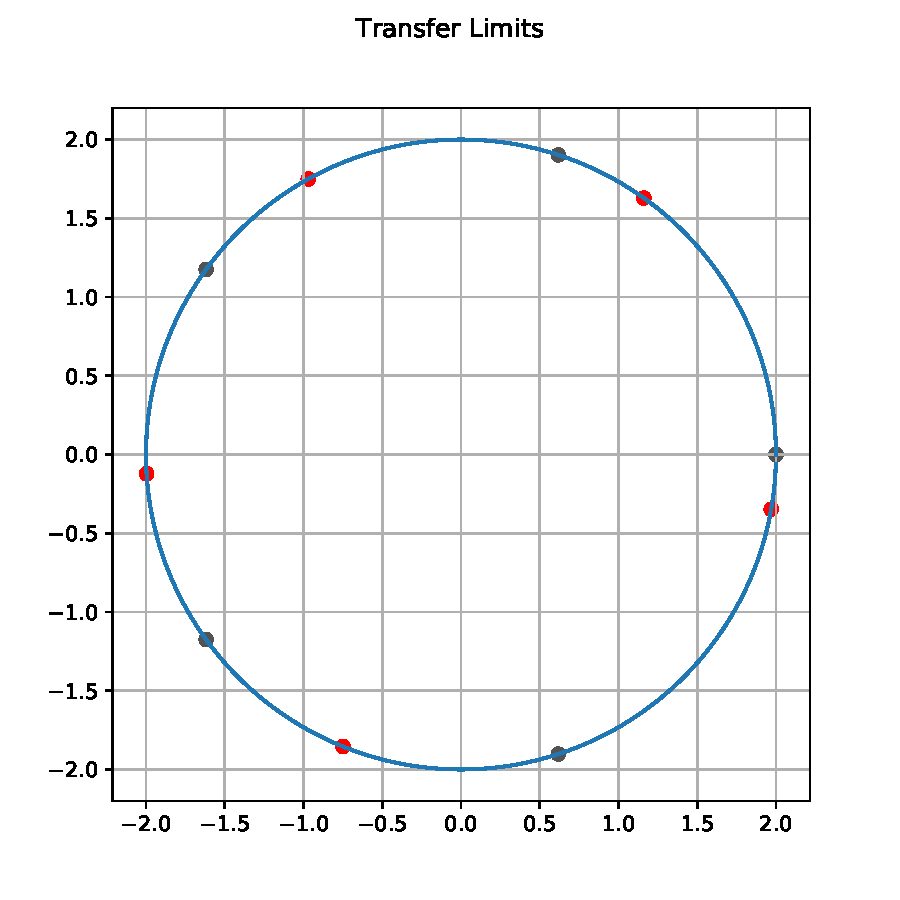
\includegraphics[scale=1.0, page=1]{visuals/Plots1}
  \caption[Area markers] {Area markers arranged on a circle} %
  \label{fig:AreaMarkers}
\end{figure*}

\clearpage

\section{Including and annotating code}
\label{sec:code}

\singlespacing
\lstinputlisting[language=python,caption={\lstname},label=lst:1, linerange={85-95}]{code/base_frame_v0.py}
\doublespacing

\section{Other formatting}
We saw in \ref{sec:figures} how to include figures.
\singlespacing
\begin{enumerate}
  \item Preprocess historic AMI data to enable study based on actual measurements.
  \item Execute OpenDSS in snapshot mode to review voltage contours at a wide
        range of operating conditions.
  \item Review the resulting patterns and place OpenDSS \emph{monitors} at
        nodes that experience greatest voltage change.
  \item Execute OpenDSS in temporal mode to collect temporal voltage recordings
        at monitored nodes.
  \item Review voltage histograms at monitored buses to quantify the frequency
        and magnitude of voltage excursions.
\end{enumerate}
\doublespacing

In the following sections, we briefly describe the tool-chains that facilitate
this process.

\clearpage

\bibliographystyle{IEEEtran} % "plain" is another option
% \bibliography{Ph2report_EC}

\clearpage

\end{document}
